% Created 2022-11-08 Tue 11:11
% Intended LaTeX compiler: xelatex
\documentclass[11pt]{article}
\usepackage{graphicx}
\usepackage{grffile}
\usepackage{longtable}
\usepackage{wrapfig}
\usepackage{rotating}
\usepackage[normalem]{ulem}
\usepackage{amsmath}
\usepackage{textcomp}
\usepackage{amssymb}
\usepackage{capt-of}
\usepackage{hyperref}
\usepackage{geometry}[margin=0.25in]

\newcommand{\bigO}[1]{\mathcal{O}\left(#1\right)}

\author{Criston}
\date{\today}
\title{Hw\#1}

\graphicspath{{./figs/}}

\begin{document}

\maketitle

\textbf{Problem 1: Nondimensionalizing Navier Stokes}

Using the nondimensionalization given, show that eq 12-14 hold.

\textbf{Solution.}

\newpage

\textbf{Problem 2:} Convert the Navier-Stokes equations to cylindrical coordinates to show that stated equations hold.

\textbf{Solution.}

\newpage

\begin{figure}
  \centering
  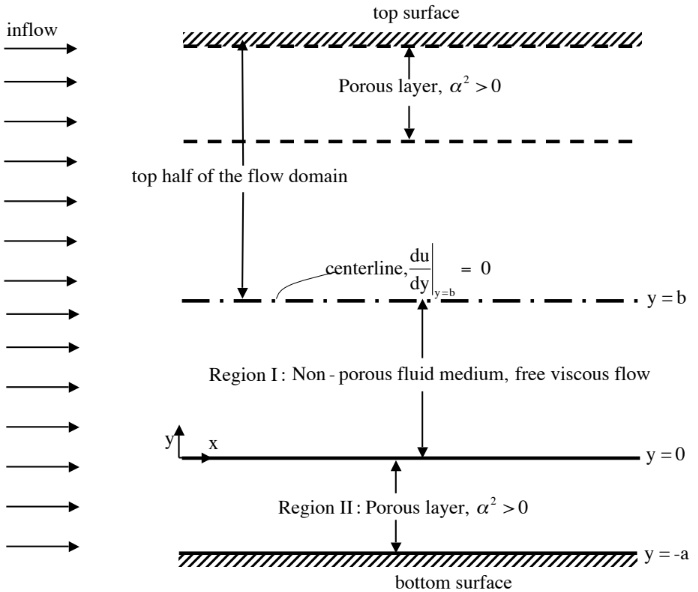
\includegraphics[width=0.5\textwidth]{prob3.png}
  \caption{Problem 3 setup}
  \label{fig:prob3}
\end{figure}

\textbf{Problem 3: Channel flow between porous layers}

Derive a simplified two-dimensional representation of flow between porous layers. Consider a channel as shown in figure \ref{fig:prob3}. The flow field is assumed symmetric about the centerline $y=b$, and the analysis should be restricted to the bottom half of the system. The flow is assumed to be steady $(u_t = 0)$ and fully developed $u_x = 0$, and zero in cross-stream direction $(v=0)$.

\textit{Region I:} Write the simplified $x$-momentum equation within the free shear flow region $\alpha^2 = 0$ along with appropriate boundary condtions.

\textit{Region II:} Write down appropriate boundary conditions and simplified equations of motion.

Solve coupled system of ODEs.


\textbf{Solution.}

\end{document}